\documentclass[12pt, a4paper]{article}
\usepackage[margin=2cm]{geometry}
\usepackage{graphicx}
\usepackage[size=footnotesize, labelfont=bf]{caption}

\author{BE19B009 - Shobhan Karthick}
\title{BT6270 Assignment 1}
\date{}

\begin{document}

\maketitle

\section{Introduction}

The Hodgkin-Huxley model clearly explains the dynamics of the ions involved in the generation of an action potential in a neuron.
The ions involved in the generation of an action potential are $ Na^{+}, K^{+}, Cl^{-} $.
When the ions reach a particular concentration on the inside of neuron and outside of the neuron, thereby reaching a particular threshold voltage of +55mV. 
Once the voltage of the neuron crosses the threshold voltage, an action potential is generated.

\section{Frequency Vs I\boldmath{$_{ext}$} plot}
\label{intro}
\begin{figure}[h] 
    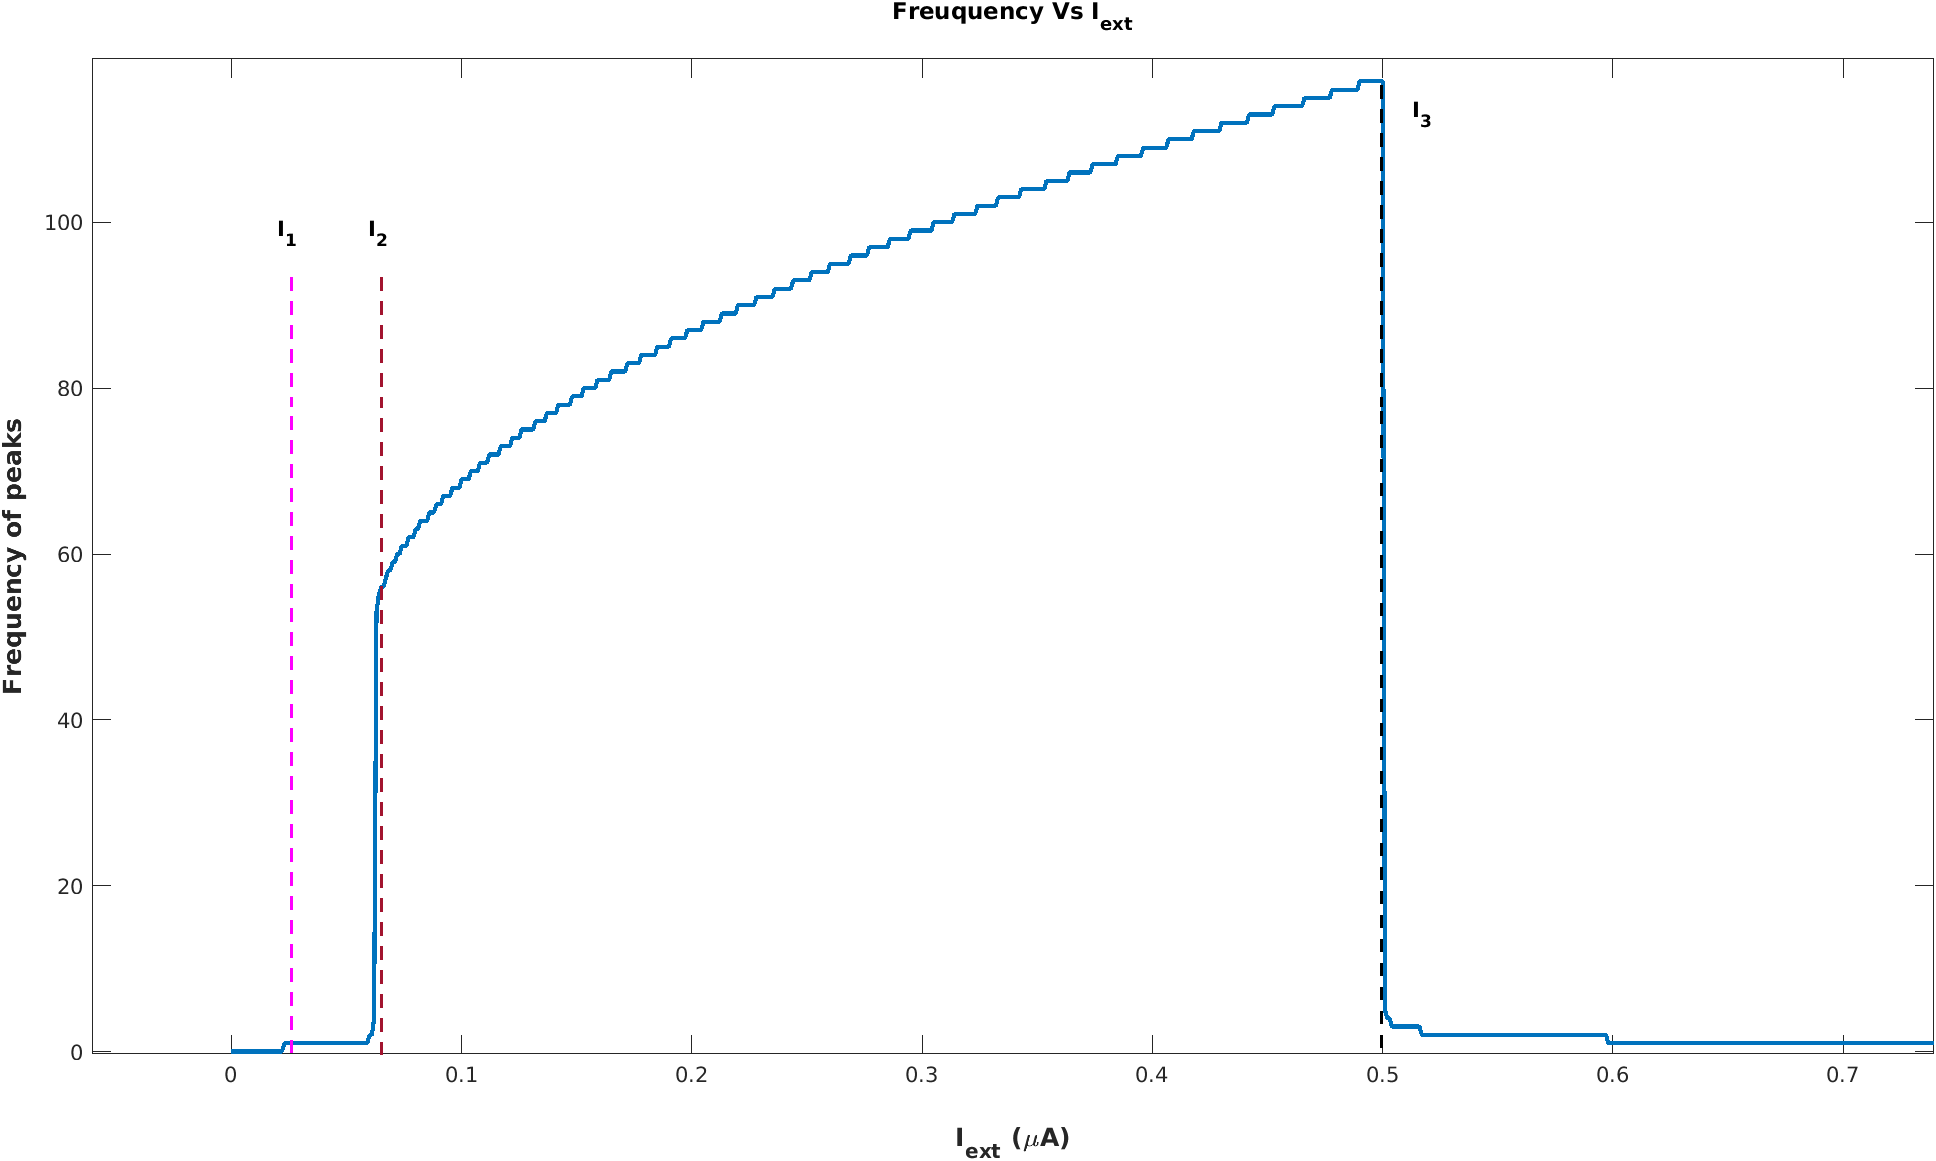
\includegraphics[width=\textwidth]{Q2_1}
    \caption{Firing rate Vs  I$ _{ext} $}
    \label{fig:Q2_1}
\end{figure}

First, in order to get a better understanding of what is happening, I modified the code such that I could visualize how the firing frequency varies with different I{$_{ext}$} ranging from 0 $ \mu A $ to 0.75 $ \mu A $ with a step size of 0.001 $ \mu A $.

This was done by adding an external for loop wrapping the already present for loop. And then, \texttt{findpeaks()} function from the \textbf{signal processsing toolbox} in MATLAB was used to find the number of action potential peaks produced for a particular I{$_{ext}$} value. And only when a local maxima is above a \textbf{threshold} value of \textbf{+7.5mv}, it is considered a peak 

Now the graph generated as a result of the previous modifications is shown in Figure \ref{fig:Q2_1}. From this graph, we can approximately interpret the values of I$_1$, I$_2$, I$_3$. Current I$_1$ is the minimum value of external current at which an action potential is generated and this can be approximated as 0.02 $ \mu A $ and further accurate analysis is done in Section \ref{I1 results}.

The \textbf{continous firing} of neuron starts at value of I$ _2 $ and ends at I$ _3 $. By interpreting the graphshown in Figure \ref{fig:Q2_1}, the values of I$ _2 $ and I$ _3 $ can be approximated to 0.06 $ \mu A $ and 0.5 $ \mu A $. Between the I$ _1 $ and I$ _2 $, there is \textbf{finite number} of action potentials generated.  And after I$ _3 $, there are almost no action potential generated by the neuron.


\section{Results with current I$_1$}
\label {I1 results}

\begin{minipage}{0.45\linewidth}
    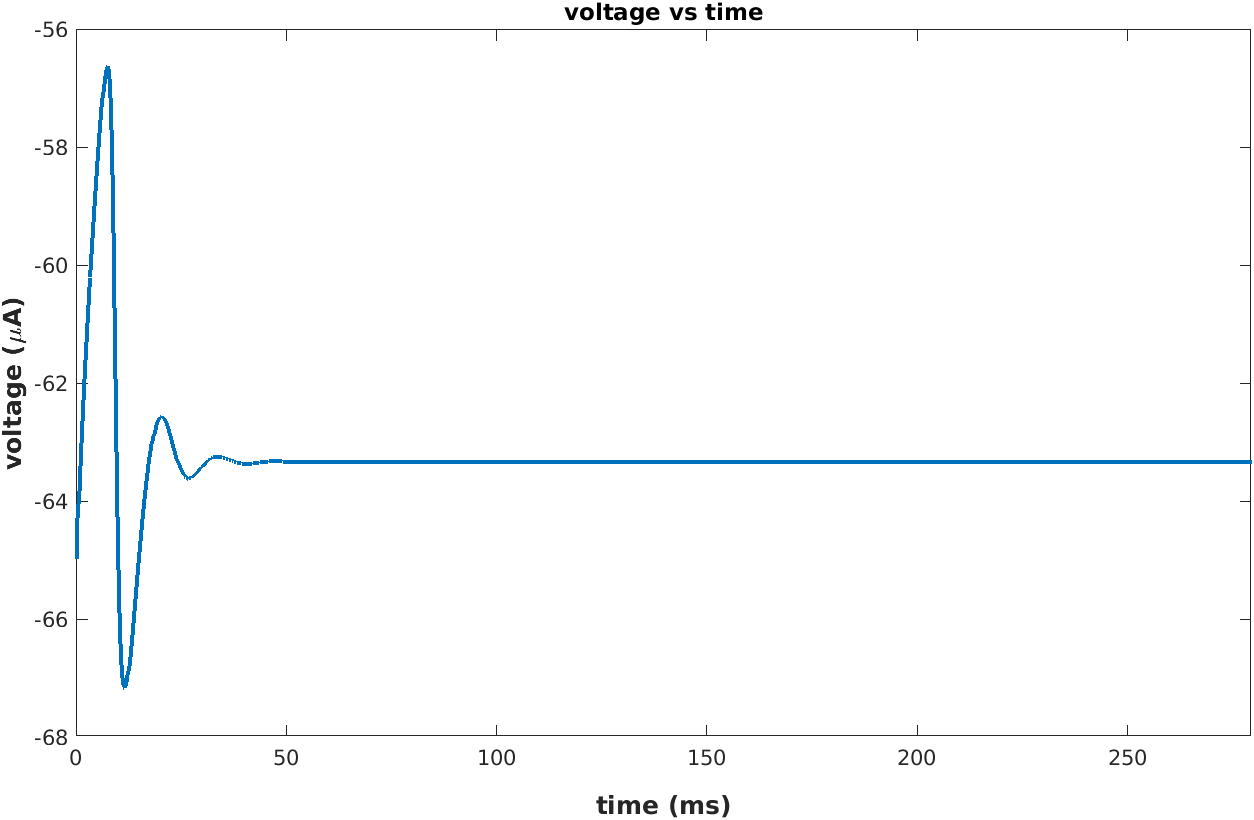
\includegraphics[width=\textwidth]{Q1_1}
    \captionof{figure}{Voltage Vs time plot at I$_{ext}$ value of 0.0223 $ \mu A $}
    \label{fig:Q1_1}
\end{minipage}
\hfill
\begin{minipage}{0.45\linewidth}
    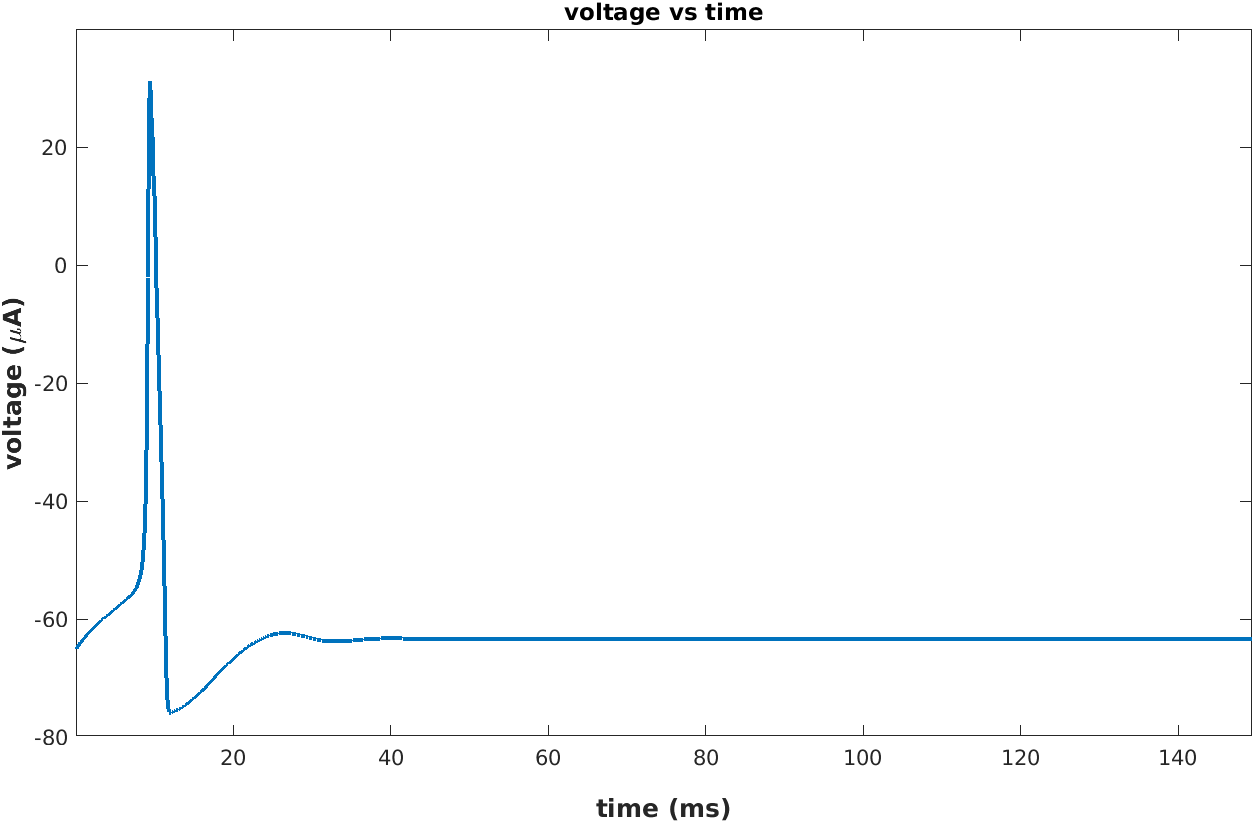
\includegraphics[width=\textwidth]{Q1_2}
    \captionof{figure}{Voltage Vs time plot at I$_{ext}$ value of 0.0224 $ \mu A $}
    \label{fig:Q1_2}
\end{minipage}

\vspace{1em}

The I$ _{ext} $ values were slowly increased from 0.02 $ \mu A $. As shown in Figure \ref{fig:Q1_1}, the plot does not look like an action potential until a I$_{ext} $ value of 0.0223 $ \mu A $. But with an increase of 0.0001 $ \mu A $, an action potential is generated as shown in Figure \ref{fig:Q1_2}.

\section{Results between current I$_1$ and I$_2$}
\label {I1-I2 results}


\begin{center}
\begin{minipage}{0.45\linewidth}
    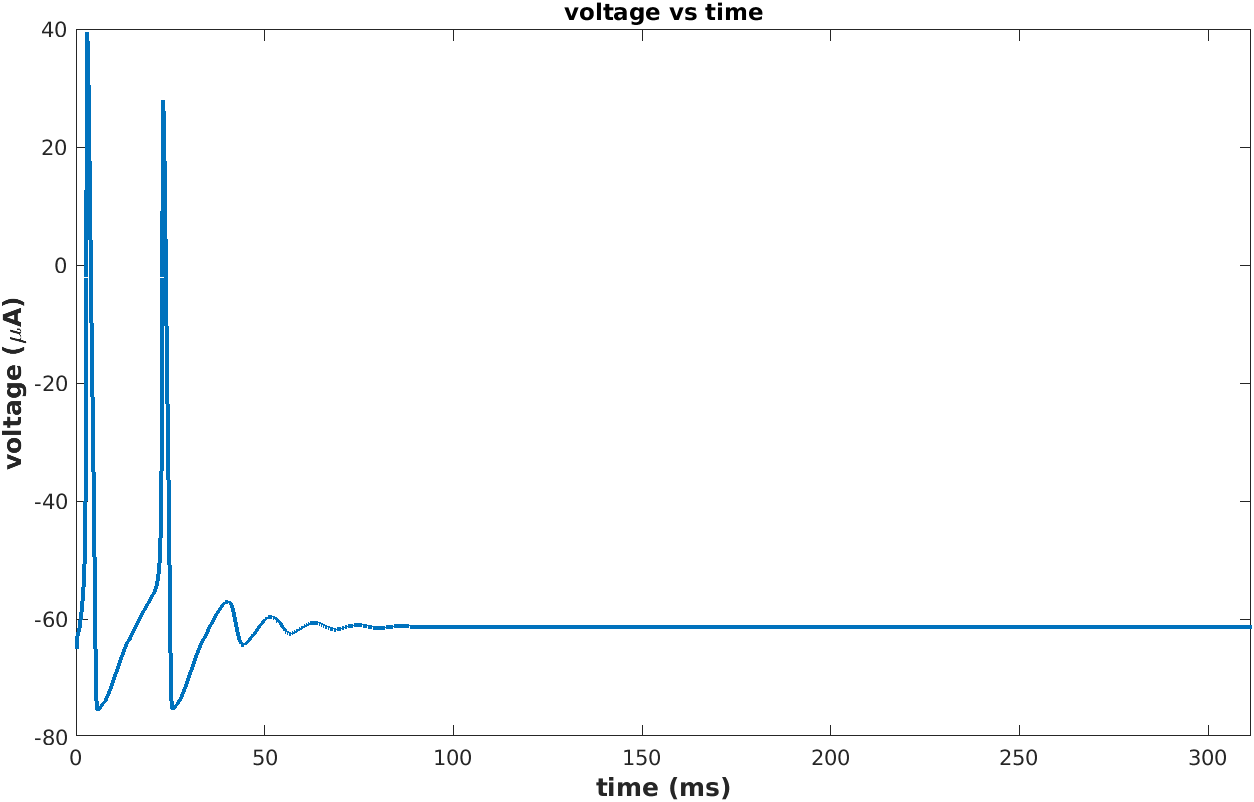
\includegraphics[width=\textwidth]{Q1_3}
    \captionof{figure}{Voltage Vs time plot at I$_{ext}$ value of 0.06 $ \mu A $}
    \label{fig:Q1_3}
\end{minipage}
\hfill
\begin{minipage}{0.45\linewidth}
    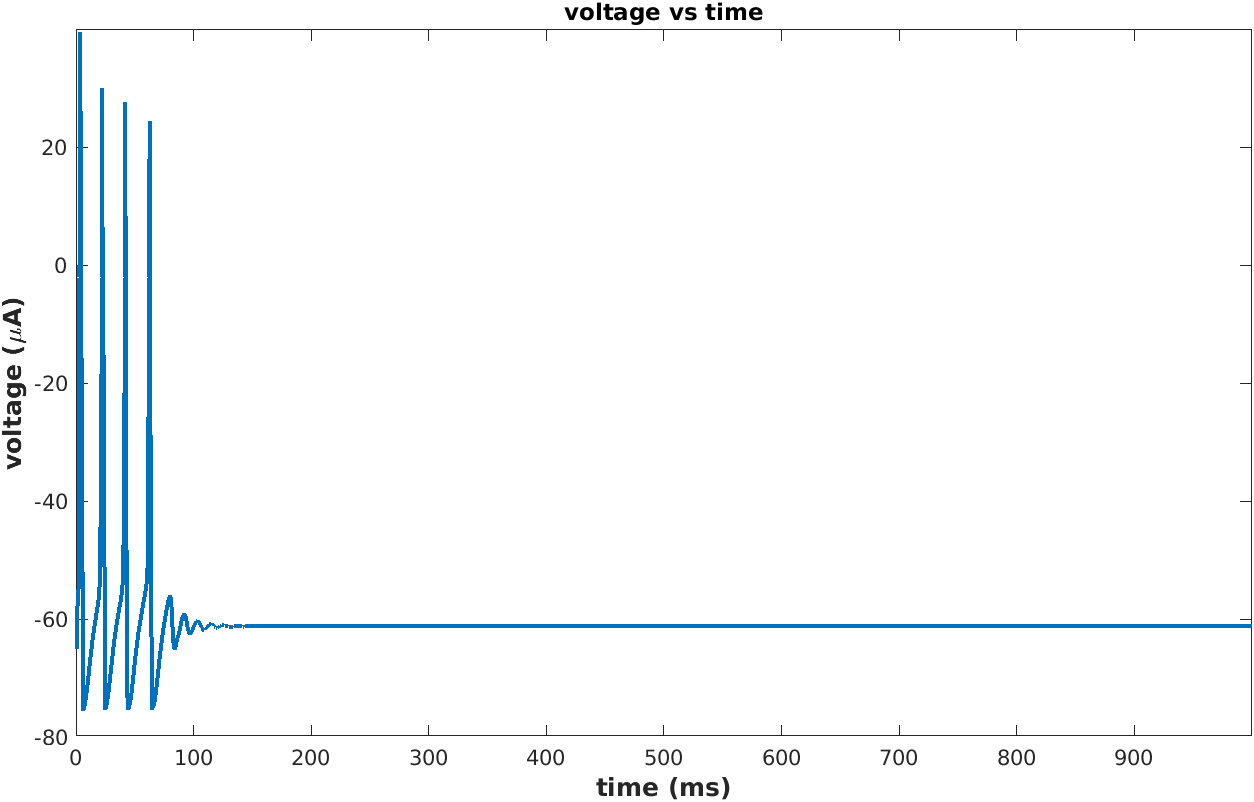
\includegraphics[width=\textwidth]{Q1_4}
    \captionof{figure}{Voltage Vs time plot at I$_{ext}$ value of 0.063 $ \mu A $}
    \label{fig:Q1_4}
\end{minipage}
\end{center}

\vspace{1em}

The second action potential starts when a current value of 0.06 $ \mu A $ is applied as shown in Figure \ref{fig:Q1_3}. The third action potential comes up at 0.063 $ \mu A $ which is shown in Figure \ref{fig:Q1_4}. This is the region in the graph with finite number of action potentials.


\section{Results between current I$_2$ and I$_3$}
\label {I2-I3 results}
\vspace{0.5em}

\begin{center}
\begin{minipage}{0.70\linewidth}
    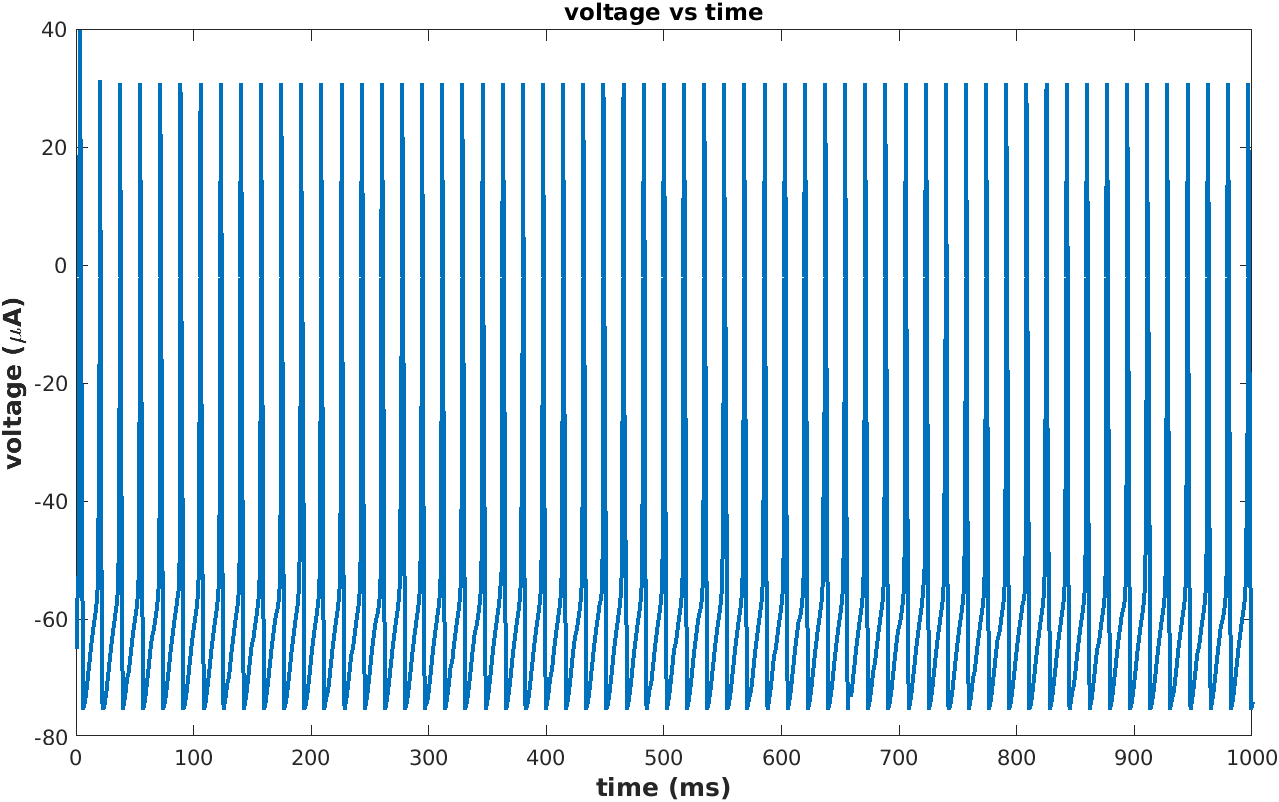
\includegraphics[width=\textwidth]{Q1_5}
    \captionof{figure}{Continous firing of action potentials}
    \label{fig:Q1_5}
\end{minipage}
\end{center}

\vspace{1em}

This region between I$_{2}$ and I$_3$ is the region with continous firing as shown in the Figure \ref{fig:Q1_5}.

\section{Results after current I$_3$ }
\label {I3 results}
\vspace{0.5em}

\begin{center}
\begin{minipage}{0.70\linewidth}
    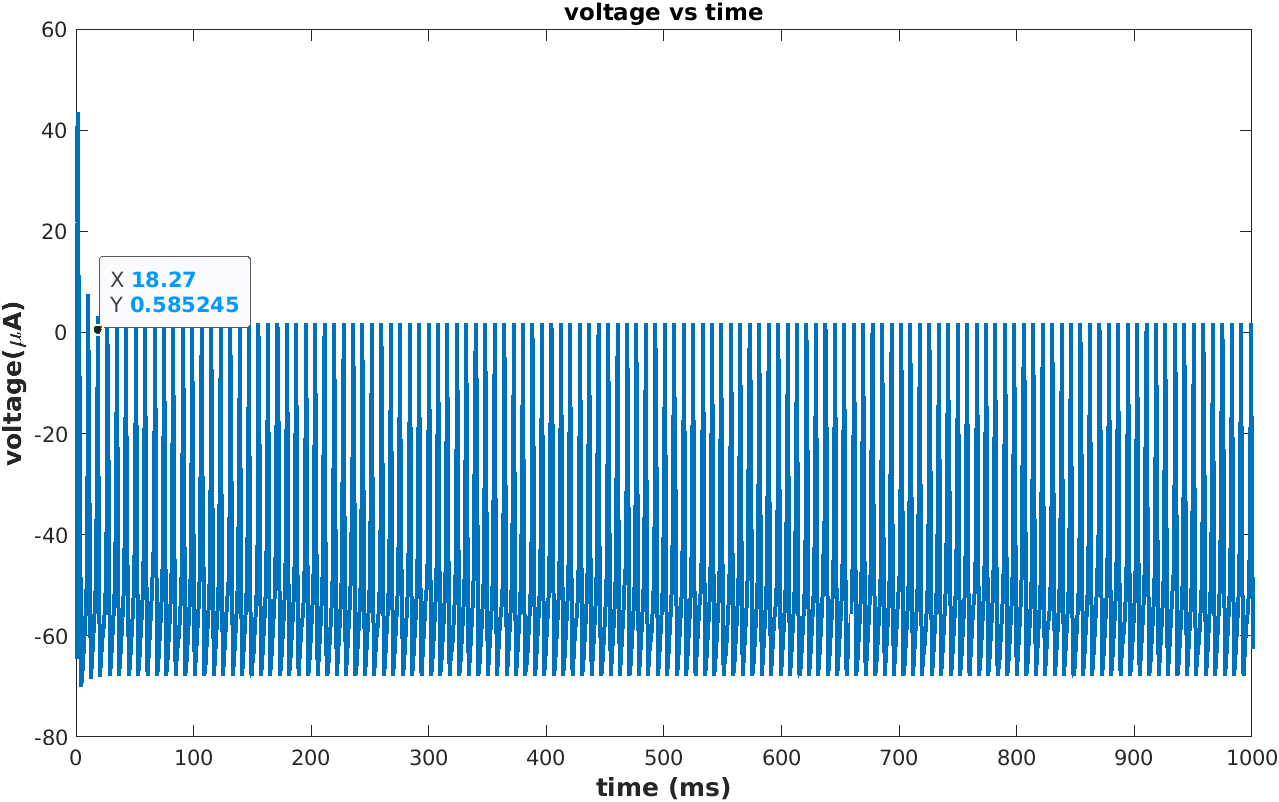
\includegraphics[width=\textwidth]{Q1_6}
    \captionof{figure}{Action potential peaks below threshold value of 7.5 $ \mu A $}
    \label{fig:Q1_6}
\end{minipage}
\end{center}

\vspace{1em}

This region after I$_{3}$ is the region with almost no action potentials as shown in Figure \ref{fig:Q2_1}. As you can see in the Figure \ref{fig:Q1_6}, there are a lot of firing happening and hence there are so many peaks, but as the data point in the figure shows, the peaks are below the \textbf{threshold} value of 7.5 $\mu A$.

\end{document}
